% Shared manuscript content for both bioRxiv and Oxford Bioinformatics versions
% This file contains only the main text content
% Metadata (title, authors, abstract, etc.) is defined in the main template files

\section{Introduction}
Reconstructing viral genomes from metagenomic sequencing data presents considerable computational challenges, particularly for viruses exhibiting extensive genetic diversity \cite{Baaijens2017-hw,Deng2021-nl,Meleshko2021-gb}. This diversity is further compounded by segmented genomes in families like influenza, rotavirus, and bunyaviruses, where individual segments can evolve under distinct selective pressures and reassort, contributing to a complex landscape for genome reconstruction. While pipelines are often designed to target specific viruses and their subtypes \cite{Shepard2016-uh}, accurate and complete genome reconstruction of samples with unknown references typically requires manual curation of contigs and reference matching \cite{Tomkins-Tinch2017-qi,Li2025-uh}. This manual curation process is time-consuming, making it impractical for large-scale metagenome studies or rapid response scenarios that involve emerging viral outbreaks of unknown origin.

To address these limitations, we developed nf-core/viralmetagenome, a comprehensive pipeline specifically designed for untargeted viral genome reconstruction. The pipeline is developed using Nextflow \cite{Di-Tommaso2017-nz} within the nf-core framework \cite{Ewels2020-kk}, ensuring reproducibility through containerization with Docker \cite{Merkel2014-hn} and Singularity \cite{Kurtzer2017-iw}, and enabling portability across computational platforms such as local desktops, high-performance clusters and cloud environments.

\section{Pipeline Description}

\href{https://github.com/nf-core/viralmetagenome}{nf-core/viralmetagenome} implements an automated workflow performing \textit{de novo} assembly, reference matching, and iterative consensus refinement for the reconstruction of  viral genomes without prior target knowledge. The pipeline consists of five major stages: read preprocessing, metagenomic diversity assessment, contig assembly and scaffolding, iterative consensus refinement with variant analysis, and quality control (Figure~\ref{fig:pipeline-workflow}). While this manuscript highlights key differences between particular tools, the pipeline offers multiple options to accommodate established user workflows and preferences. Tool details are in Supplementary Table 1.

\begin{figure*}[htbp]
    \centering
    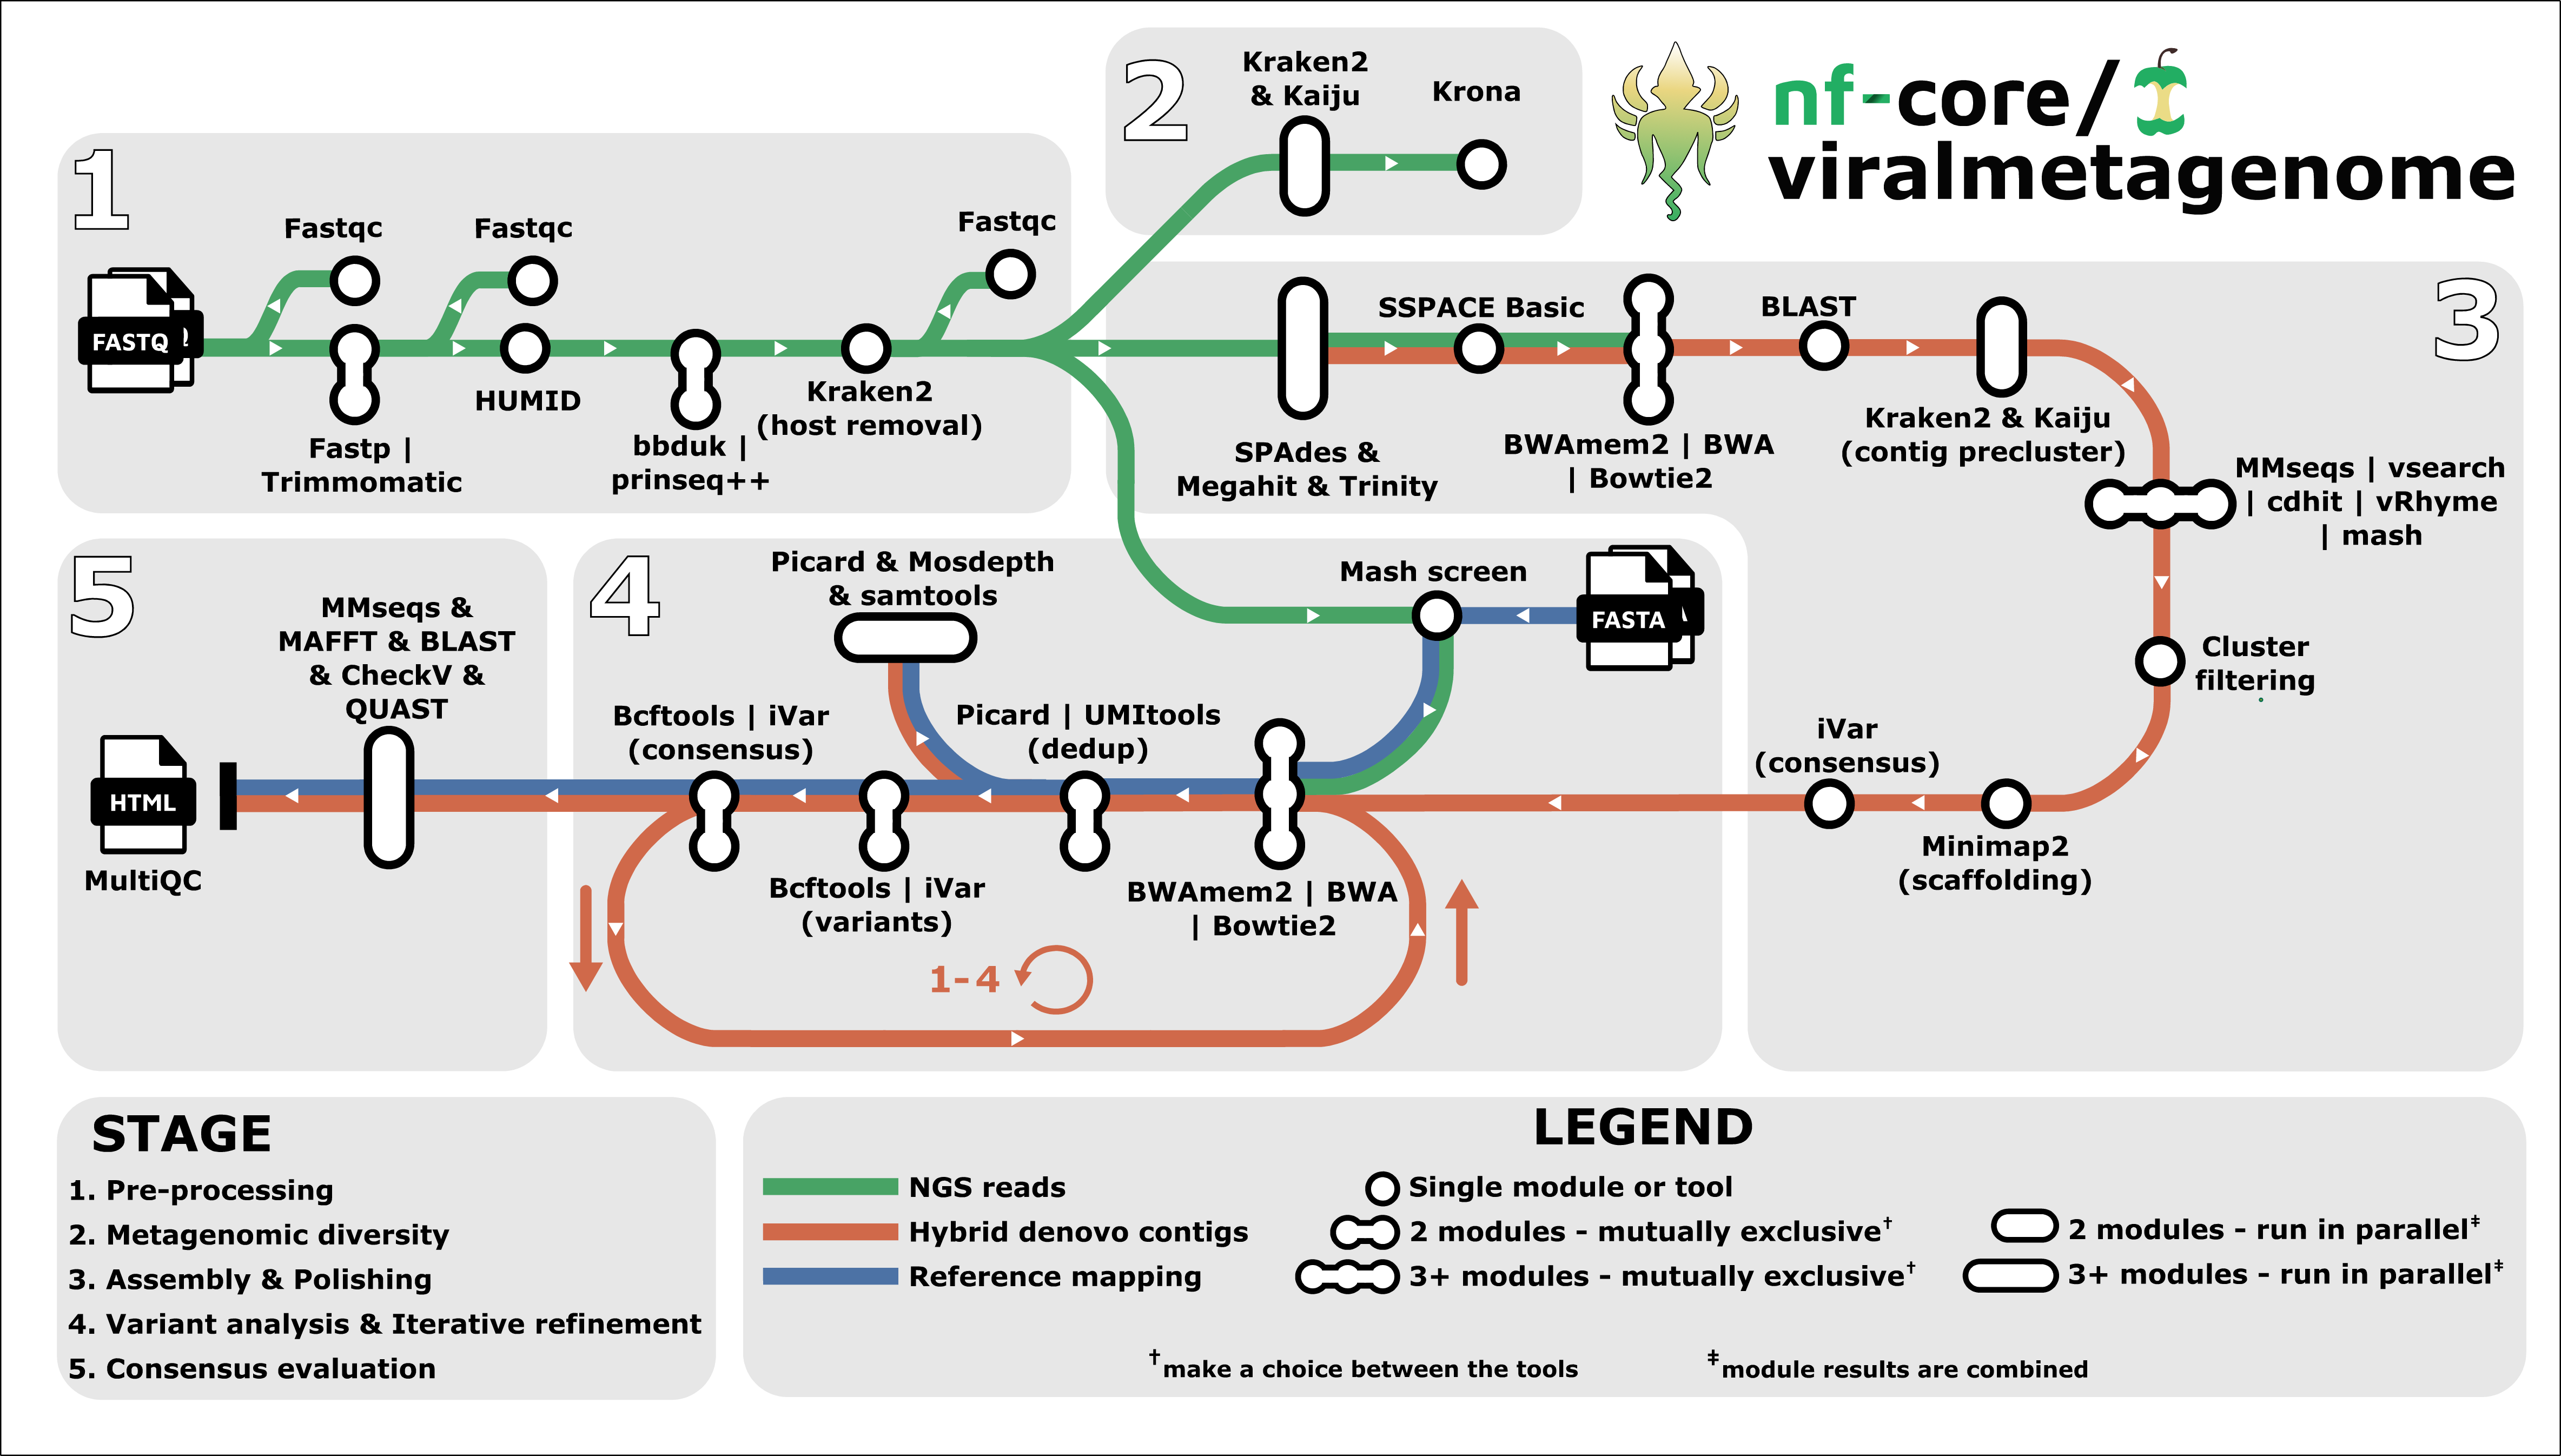
\includegraphics[width=1\textwidth]{Fig/fig1.png}
    \caption{Visual overview of the nf-core/viralmetagenome pipeline for untargeted viral genome reconstruction. nf-core/viralmetagenome processes short-read data through pre-processing, metagenomic diversity assessment, \textit{de novo} assembly with multiple assemblers, scaffolding with automated reference identification and contig taxonomy-guided clustering, and iterative consensus refinement through read mapping and variant calling. Quality control metrics, assembly statistics, and coverage data are integrated into interactive MultiQC reports and standardised overview tables for downstream analysis.}
    \label{fig:pipeline-workflow}
\end{figure*}


\subsection{Read preprocessing}

Input reads provided via sample sheets containing sample names and short-read FASTQ paths are   preprocessed using FastQC and have their adapter trimmed with Fastp \cite{Chen2018-tu} (default) or Trimmomatic \cite{Bolger2014-si}. Fastp is overall faster and has automated adapter detection and trimming \cite{Chen2018-tu}. UMI deduplication is implemented using HUMID \cite{LarosUnknown-nx} and UMI-tools \cite{Smith2017-nk} once reads are mapped to a reference. Multiple sequencing runs are merged after trimming by specifying merge group identifiers in the sample sheet. Complexity filtering with BBduk \cite{BushnellUnknown-qy} or prinseq++ \cite{Cantu2019-vs} removes low-complexity sequences containing repetitive elements. Host removal uses Kraken2 \cite{Wood2019-jl} against user-specified databases (default: human genome subset). However, users are encouraged to employ more comprehensive databases, including complete host genome and transcriptome (human and otherwise), common sequencer contaminants, and bacterial genomes, to ensure thorough decontamination \cite{Forbes2025-mv}.

\subsection{Metagenomic diversity assessment}

Taxonomic classification of preprocessed reads is performed using two complementary approaches - Kaiju \cite{Menzel2016-tz} and Kraken2 \cite{Wood2019-jl} - to maximise detection sensitivity across diverse viral families. Results from both classifiers are visualised using Krona \cite{Ondov2011-yp}.

\subsection{{\it De novo} assembly and clustering}

The assembly workflow implements multi-assembler approaches followed by clustering and scaffolding. \textit{De novo} assembly is performed using SPAdes \cite{Meleshko2021-gb} (RNAviral mode), MEGAHIT \cite{Li2016-sd}, and Trinity \cite{Grabherr2011-ef}, capitalizing on distinct algorithmic strengths to maximise genome recovery across diverse viral families and variable read depths. Contigs can optionally be extended with SSPACE Basic \cite{Boetzer2011-dh}.

Reference identification uses BLASTn \cite{Altschul1990-sy} against the Reference Viral Database (RVDB) \cite{Goodacre2018-dw}, retaining top five hits to facilitate identification of related genomic segments and appropriate reference sequences for contig scaffolding and clustering.

Clustering employs two stages: taxonomic pre-clustering using Kraken2 \cite{Wood2019-jl} and Kaiju \cite{Menzel2016-tz}. For more efficient targeted analyses, the user can opt to focus on specific taxonomic clades. Subsequent nucleotide similarity clustering is done with CD-HIT-EST \cite{Li2006-nj}, VSEARCH \cite{Rognes2016-ju}, MMseqs2 \cite{Steinegger2017-ci}, vRhyme \cite{Kieft2022-km}, or Mash \cite{Ondov2019-bo}. All tools are valid options, though performance may vary depending on the dataset; for comprehensive benchmarking, we refer to Zielezinski et al. \cite{Zielezinski2025-vl} and Steinegger and Söding \cite{Steinegger2017-ci}.

As an optional filtering step of contig clusters, after assembly and extension, reads can be mapped to all contigs using BWAmem2 \cite{Vasimuddin2019-rb} (default), BWA \cite{Li2013-pp}, or Bowtie2 \cite{Langmead2019-wx}. Clusters are filtered based on the cumulated percentage of reads mapped to the contigs of a cluster. By filtering clusters, low-coverage assemblies can be identified that likely represent assembly artefacts.

For the final scaffolding step, all cluster members are mapped to the cluster representative or centroid using Minimap2 \cite{Li2018-gi}, followed by consensus calling with iVar \cite{Grubaugh2019-xd} to generate reference-assisted assemblies. Regions with zero coverage depth can optionally be represented by the reference genome to produce a more complete scaffold genome for consensus calling.

\subsection{Iterative consensus refinement and variant calling}

The consensus module supports external reference-based analysis and scaffold refinement. Users can provide a separate reference genome or reference set for each sample with \texttt{--mapping\_constraints}; when a reference set is provided, the most similar can be selected using Mash \cite{Ondov2019-bo}.

Scaffold refinement performs up to 4 iterative cycles (default 2). Each iteration maps reads using BWAmem2 \cite{Vasimuddin2019-rb}, BWA \cite{Li2013-pp}, or Bowtie2 \cite{Langmead2019-wx} to the consensus, followed by variant calling with BCFtools \cite{Danecek2021-je} or iVar \cite{Grubaugh2019-xd}. Benchmarking by Bassano et al. \cite{Bassano2022-cl} showed that BCFtools outperformed iVar in precision and recall. iVar detects more low-frequency variants, resulting in an increased false positive rate but decreases the number of identified false negatives \cite{Bassano2022-cl}. Users are recommended to consider prioritising sensitivity or specificity when selecting the variant caller.

Optional deduplication can be performed using Picard or when UMI’s are available with UMI-tools \cite{Smith2017-nk}. Mapping statistics are generated using samtools (flagstat, idxstats, stats) \cite{Danecek2021-je}, Picard CollectMultipleMetrics \cite{Broad-Institute2019-rv}, and coverage statistics with mosdepth \cite{Pedersen2018-mu}.

\subsection{Consensus Quality Control}

Quality control employs CheckV \cite{Nayfach2021-wl} for completeness estimates, BLASTn \cite{Altschul1990-sy} for reference similarity, and MMseqs2 \cite{Steinegger2017-ci} against the annotated database Virosaurus \cite{Gleizes2020-rq}. These analyses enable species identification, genomic segment classification, host association determination, and extraction of additional metadata embedded within the reference databases.

The refinement progression is evaluated through sequence alignment with MAFFT \cite{Katoh2002-ox}, which compares final consensus genomes against \textit{de novo} contigs, intermediate consensus sequences from iterative cycles, and the scaffolding reference. All tool metrics are compiled into an interactive MultiQC report \cite{Ewels2016-hs}. Additionally, key metrics are extracted from the MultiQC report and compiled into standalone overview tables to facilitate downstream analysis across all processed samples.

\section{Applications}

To assess the performance of nf-core/viralmetagenome under challenging scenarios, we simulated coinfection scenarios by mixing paired-end reads from public HIV-1 genomes with varying diversity (80-99\% similarity), resulting in 13 samples (See supplementary table 2). Nf-core/viralmetagenome successfully identified coinfections in all mixed samples when genetic similarity was low to moderate ($\leq$ 96.7\% ANI).

We investigated how reference genome selection affects consensus accuracy. While similar references ($\geq$ 96\%) minimally impact consensus quality, divergent references introduce up to 187 nucleotide mismatches (Figure~\ref{fig:reference-influence}). These findings underscore the critical importance of appropriate reference selection for scaffolding and sequence alignment procedures. Nf-core/viralmetagenome addresses this challenge by automatically selecting the most appropriate reference genome based on sequence similarity; however, when no suitable genome is found in the supplied database, the contigs are scaffolded to a \textit{de novo} contig (specifically, the cluster representative), ensuring that the final consensus genomes are as accurate as possible.

\begin{figure}[htbp]
    \centering
    \includegraphics[width=0.5\textwidth]{Fig/fig2.png}
    \caption{Boxplot of maximum observed differences between consensus sequences generated with different reference genomes during scaffolding. Mean highlighted by a diamond.}
    \label{fig:reference-influence}
\end{figure}

We validated nf-core/viralmetagenome performance on real metagenomic samples spanning human and plant pathogens. Here, the pipeline successfully generated high-quality or near-complete genomes across viral families including segmented (Lassa virus, Orthonairovirus, Tomato spotted wilt tospovirus) and non-segmented viruses (SARS-CoV-2, West Nile virus, Potato virus Y,Youcai mosaic virus, and Monkeypox virus).

Processing 28 samples (supplementary methods) required 412 CPU hours and a maximum of 79GB RAM on an HPC, excluding taxonomic classification steps. The automated reference selection during scaffolding offers substantial improvements over manual curation by reducing processing time while preserving reconstruction accuracy. Performance correlates strongly with reference database comprehensiveness as consensus genomes tended to be more complete and similar to the true consensus sequence when scaffolding reference was closer to the true viral genome. This emphasizes the need to keep databases like RVDB \cite{Goodacre2018-dw} and Virosaurus \cite{Gleizes2020-rq} up-to-date. Since nf-core/viralmetagenome is primarily designed for eukaryotic viruses, bacteriophage analysis requires different approaches and users are encouraged to explore pipelines targeting phages such as VIRify \cite{Rangel-Pineros2022-wv}, VIBRANT \cite{Kieft2020-aq}, VirSorter2 \cite{Guo2021-rf}.


\section{Conclusion}

nf-core/viralmetagenome addresses a critical need in viral genomics by providing an automated, scalable solution for untargeted viral genome reconstruction. The pipeline successfully automates the traditionally time-consuming and manual execution process of viral genome assembly from short-read metagenomic data through its integrated workflow of \textit{de novo} contig assembly, automated reference selection, clustering algorithms, and iterative refinement strategies.

Our validation demonstrates the pipeline's broad applicability across diverse eukaryotic viral families, achieving high-quality genome reconstruction while ensuring reproducibility and ease of deployment across different computational environments.

As viral surveillance and outbreak response increasingly rely on metagenomic sequencing, automated pipelines like nf-core/viralmetagenome will be essential for the timely identification of pathogen strains. The pipeline represents a significant step forward in making viral genome reconstruction accessible to researchers without requiring extensive bioinformatics expertise, facilitating broader adoption of metagenomic approaches in viral research and public health applications.


\section*{Acknowledgments}
 J.K, P.L. and L.E.K  acknowledge support from the Research Foundation - Flanders (Fonds voor Wetenschappelijk Onderzoek – Vlaanderen, G005323N and G051322N, 1SH2V24N, 12X9222N).

\section*{Author Contributions}
J.K. designed and implemented the pipeline, performed validation analyses, and wrote the manuscript. P.L. and L.E.K. supervised the project and provided critical feedback. The nf-core community contributed to maintaining the pipeline. All authors reviewed and approved the final manuscript.

\section*{Data Availability}
The nf-core/viralmetagenome pipeline is freely available at https://github.com/nf-core/viralmetagenome.
The raw data and analysis code is available on https://github.com/Joon-Klaps/nf-core-viralmetagenome-manuscript/.

\section*{Conflict of Interest}
The authors declare no competing interests.

